\documentclass[11pt,letterpaper]{report}
\usepackage[utf8]{inputenc}
\usepackage[english]{babel}
\usepackage{amsmath}
\usepackage{amsfonts}
\usepackage{amssymb}
\usepackage{graphicx}
\usepackage{xcolor}
\usepackage{siunitx}
\usepackage{upgreek}
\usepackage{apacite}
\usepackage{booktabs}
\usepackage{ntheorem}
\usepackage{subcaption}
\usepackage{enumitem}
\usepackage{gensymb}
\usepackage[ruled,vlined, linesnumbered]{algorithm2e}
\graphicspath{ {./Figures/} }
\newtheorem{hyp}{Hypothesis}
\usepackage[left=2cm,right=2cm,top=2cm,bottom=2cm]{geometry}
\author{
	Kho, Lee\\
	\textit{ltk224}
	\and
	Peeters, Jonas\\
	\textit{jp5642}
}
\title{DS-GA 1013: Project\\Intelligible Principal Component Analysis}

\usepackage[strings]{underscore}
\usepackage{fancyhdr}
\fancypagestyle{plain}{
    \fancyhf{}
    \lhead{Kho \& Peeters}
    \chead{\thepage}
    \rhead{DS-GS 1013}
}
\pagestyle{plain}

\setlength\parindent{0pt}
\allowdisplaybreaks

%% Probability operators and functions
%
% \def \P{\mathrm{P}}
\def \P{\mathrm{P}}
\def \E{\mathrm{E}}
\def \Var{\mathrm{Var}}
\let\var\Var
\def \Cov {\mathrm{Cov}} \let\cov\Cov
\def \Corr {\mathrm{Corr}}
\def \MSE {\mathrm{MSE}} \let\mse\MSE
\def \sgn {\mathrm{sgn}}
\def \R {\mathbb{R}}
\def \C {\mathbb{C}}
\def \N {\mathbb{N}}
\def \Z {\mathbb{Z}}
\def \cV {\mathcal{V}}
\def \cS {\mathcal{S}}
\newcommand{\RR}{\ensuremath{\mathbb{R}}}
\DeclareMathOperator*{\argmin}{arg\,min}
\DeclareMathOperator*{\argmax}{arg\,max}
\newcommand{\red}[1]{\textcolor{red}{#1}}
\newcommand{\blue}[1]{\textcolor{blue}{#1}}
\newcommand{\green}[1]{\textcolor{ForestGreen}{ #1}}
\newcommand{\fuchsia}[1]{\textcolor{RoyalPurple}{ #1}}
\DeclareMathOperator{\Norm}{\mathcal{N}}

%
%% Probability distributions
%
%\def \Bern    {\mathrm{Bern}}
%\def \Binom   {\mathrm{Binom}}
%\def \Exp     {\mathrm{Exp}}
%\def \Geom    {\mathrm{Geom}}
%\def \Norm    {\mathcal{N}}
%\def \Poisson {\mathrm{Poisson}}
%\def \Unif    {\mathrm {U}}
%
\newcommand{\bdb}[1]{\textcolor{red}{#1}}

\newcommand{\ml}[1]{\mathcal{ #1 } }
\newcommand{\wh}[1]{\widehat{ #1 } }
\newcommand{\wt}[1]{\widetilde{ #1 } }
\newcommand{\conj}[1]{\overline{ #1 } }
\newcommand{\rnd}[1]{\tilde{ #1 } }
\newcommand{\rv}[1]{ \rnd{ #1}  }
\newcommand{\rx}{\rnd{ x}  }
\newcommand{\ry}{\rnd{ y}  }
\newcommand{\ra}{\rnd{ a}  }
\newcommand{\rb}{\rnd{ b}  }
\newcommand{\rz}{\rnd{ z}  }
\newcommand{\rpc}{\widetilde{ pc}  }
\newcommand{\rndvec}[1]{\vec{\rnd{#1}}}


\def \cnd {\, | \,}
\def \Id { I }
\def \J {\mathbf{1}\mathbf{1}^T}

\newcommand{\op}[1]{\operatorname{#1}}
\newcommand{\setdef}[2]{ := \keys{ #1 \; | \; #2 } }
\newcommand{\set}[2]{ \keys{ #1 \; | \; #2 } }
\newcommand{\sign}[1]{\op{sign}\left( #1 \right) }
\newcommand{\trace}[1]{\op{tr}\left( #1 \right) }
\newcommand{\tr}[1]{\op{tr}\left( #1 \right) }
\newcommand{\inv}[1]{\left( #1 \right)^{-1} }
\newcommand{\abs}[1]{\left| #1 \right|}
\newcommand{\sabs}[1]{| #1 |}
\newcommand{\keys}[1]{\left\{ #1 \right\}}
\newcommand{\sqbr}[1]{\left[ #1 \right]}
\newcommand{\sbrac}[1]{ ( #1 ) }
\newcommand{\brac}[1]{\left( #1 \right) }
\newcommand{\bbrac}[1]{\big( #1 \big) }
\newcommand{\Bbrac}[1]{\Big( #1 \Big)}
\newcommand{\BBbrac}[1]{\BIG( #1 \Big)}
\newcommand{\MAT}[1]{\begin{bmatrix} #1 \end{bmatrix}}
\newcommand{\sMAT}[1]{\left(\begin{smallmatrix} #1 \end{smallmatrix}\right)}
\newcommand{\sMATn}[1]{\begin{smallmatrix} #1 \end{smallmatrix}}
\newcommand{\PROD}[2]{\left \langle #1, #2\right \rangle}
\newcommand{\PRODs}[2]{\langle #1, #2 \rangle}
\newcommand{\der}[2]{\frac{\text{d}#2}{\text{d}#1}}
\newcommand{\pder}[2]{\frac{\partial#2}{\partial#1}}
\newcommand{\derTwo}[2]{\frac{\text{d}^2#2}{\text{d}#1^2}}
\newcommand{\ceil}[1]{\lceil #1 \rceil}
\newcommand{\Imag}[1]{\op{Im}\brac{ #1 }}
\newcommand{\Real}[1]{\op{Re}\brac{ #1 }}
\newcommand{\norm}[1]{\left|\left| #1 \right|\right| }
\newcommand{\norms}[1]{ \| #1 \|  }
\newcommand{\normProd}[1]{\left|\left| #1 \right|\right| _{\PROD{\cdot}{\cdot}} }
\newcommand{\normTwo}[1]{\left|\left| #1 \right|\right| _{2} }
\newcommand{\normTwos}[1]{ \| #1  \| _{2} }
\newcommand{\normZero}[1]{\left|\left| #1 \right|\right| _{0} }
\newcommand{\normTV}[1]{\left|\left| #1 \right|\right|  _{ \op{TV}  } }% _{\op{c} \ell_1} }
\newcommand{\normOne}[1]{\left|\left| #1 \right|\right| _{1} }
\newcommand{\normOnes}[1]{\| #1 \| _{1} }
\newcommand{\normOneTwo}[1]{\left|\left| #1 \right|\right| _{1,2} }
\newcommand{\normF}[1]{\left|\left| #1 \right|\right| _{\op{F}} }
\newcommand{\normLTwo}[1]{\left|\left| #1 \right|\right| _{\ml{L}_2} }
\newcommand{\normNuc}[1]{\left|\left| #1 \right|\right| _{\ast} }
\newcommand{\normOp}[1]{\left|\left| #1 \right|\right|  }
\newcommand{\normInf}[1]{\left|\left| #1 \right|\right| _{\infty}  }
\newcommand{\proj}[1]{\mathcal{P}_{#1} \, }
\newcommand{\diff}[1]{ \, \text{d}#1 }
\newcommand{\vc}[1]{\boldsymbol{\vec{#1}}}
\newcommand{\rc}[1]{\boldsymbol{#1}}
\newcommand{\vx}{\vec{x}}
\newcommand{\vy}{\vec{y}}
\newcommand{\vz}{\vec{z}}
\newcommand{\vu}{\vec{u}}
\newcommand{\vv}{\vec{v}}
\newcommand{\vb}{\vec{\beta}}
\newcommand{\va}{\vec{\alpha}}
\newcommand{\vaa}{\vec{a}}
\newcommand{\vbb}{\vec{b}}
\newcommand{\vg}{\vec{g}}
\newcommand{\vw}{\vec{w}}
\newcommand{\vh}{\vec{h}}
\newcommand{\vnu}{\vec{\nu}}
\newcommand{\rvnu}{\vc{\nu}}
\newcommand{\vbeta}{\vec{\beta}}
\newcommand{\valpha}{\vec{\alpha}}
\newcommand{\vgamma}{\vec{\gamma}}
\newcommand{\veta}{\vec{\eta}}
\newcommand{\rw}{\rnd{w}}
\newcommand{\rvv}{\rndvec{v}}
\newcommand{\rvw}{\rndvec{w}}
\newcommand{\rvx}{\rndvec{x}}
\newcommand{\rvy}{\rndvec{y}}
\newcommand{\rvz}{\rndvec{z}}
\newcommand{\rvX}{\rndvec{X}}

\newtheorem{theorem}{Theorem}[section]
% \declaretheorem[style=plain,qed=$\square$]{theorem}
\newtheorem{corollary}[theorem]{Corollary}
\newtheorem{definition}[theorem]{Definition}
\newtheorem{lemma}[theorem]{Lemma}
\newtheorem{remark}[theorem]{Remark}
\newtheorem{algorithm}[theorem]{Algorithm}

% \theoremstyle{definition}
%\newtheorem{example}[proof]{Example}
%\declaretheorem[style=definition,qed=$\triangle$,sibling=definition]{example}
%\declaretheorem[style=definition,qed=$\bigcirc$,sibling=definition]{application}

%
%% Typographic tweaks and miscellaneous
%\newcommand{\sfrac}[2]{\mbox{\small$\displaystyle\frac{#1}{#2}$}}
%\newcommand{\suchthat}{\kern0.1em{:}\kern0.3em}
%\newcommand{\qqquad}{\kern3em}
%\newcommand{\cond}{\,|\,}
%\def\Matlab{\textsc{Matlab}}
%\newcommand{\displayskip}[1]{\abovedisplayskip #1\belowdisplayskip #1}
%\newcommand{\term}[1]{\emph{#1}}
%\renewcommand{\implies}{\;\Rightarrow\;}

% mathcal
\newcommand{\cF}{\mathcal{F}}
\newcommand{\cN}{\mathcal{N}}
\newcommand{\cT}{\mathcal{T}}
\newcommand{\cC}{\mathcal{C}}
\newcommand{\cZ}{\mathcal{Z}}
\newcommand{\cD}{\mathcal{D}}
\newcommand{\cB}{\mathcal{B}}

% Transpose 
\def\sT{{\sf T}}
\def\deg{{\rm deg}}

% Trace and Variance
\def\Tr{{{\rm Tr}}}
\def\Var{{{\rm Var}}}
\def\Cov{{{\rm Cov}}}


\def\eps{{\varepsilon}}

% Linear algebra
\def\Span{{{\rm Span}}}
\def\dim{{{\rm dim}}}
\def\Ker{{{\rm Ker}}}
\def\Im{{{\rm Im}}}
\def\Id{{{\rm Id}}}
\def\rank{{{\rm rank}}}
\def\Sp{{{\rm Sp}}}
\def\Diag{{{\rm Diag}}}

% Mean-square errors
\def\MMSE{{{\rm MMSE}}}
\def\MSE{{{\rm MSE}}}
\def\DMSE{{{\rm DMSE}}}
\def\mmse{{{\rm mmse}}}

% Probability
\renewcommand{\P}{\mathbb{P}}
\newcommand{\iid}{\overset{\text{\tiny i.i.d.}}{\sim}}
\def\Dtv{\text{D}_{\text{\scriptsize TV}}}
\def\Dkl{\text{D}_{\text{\scriptsize KL}}}

% Usual laws
\def\Poi{\text{Poi}}
\def\Pois{\text{Pois}}
\def\Bin{\text{Bin}}
\def\Ber{\text{Ber}}
\def\Unif{\text{Unif}}

% Double brackets
\def\llbracket{[\hspace{-.10em} [ }
\def\rrbracket{ ] \hspace{-.10em}] }

\def\1{\mathds{1}}

% Math-bold
\newcommand{\bbf}[1]{\mathbf{#1}}

% hat
\newcommand{\what}[1]{\widehat{#1}}

% widebar
\DeclareFontFamily{U}{mathx}{\hyphenchar\font45}
\DeclareFontShape{U}{mathx}{m}{n}{<-> mathx10}{}
\DeclareSymbolFont{mathx}{U}{mathx}{m}{n}
\DeclareMathAccent{\widebar}{0}{mathx}{"73}

% def eq
\newcommand{\defeq}{\overset{\rm def}{=}}

% Frobenius norm
\newcommand{\frob}[1]{\langle #1 \rangle_F }

% Vectorized matrix
\def\vect{{\rm vec}}

\makeatletter
\def\@makechapterhead#1{%
  %%%%\vspace*{50\p@}% %%% removed!
  {\parindent \z@ \raggedright \normalfont
    \ifnum \c@secnumdepth >\m@ne
        \huge\bfseries \@chapapp\space \thechapter
        \par\nobreak
        \vskip 20\p@
    \fi
    \interlinepenalty\@M
    \Huge \bfseries #1\par\nobreak
    \vskip 40\p@
  }}
\def\@makeschapterhead#1{%
  %%%%%\vspace*{50\p@}% %%% removed!
  {\parindent \z@ \raggedright
    \normalfont
    \interlinepenalty\@M
    \Huge \bfseries  #1\par\nobreak
    \vskip 40\p@
  }}
\makeatother

\begin{document}
\maketitle
\section*{Introduction}

Principal component analysis (PCA) is a popular dimension-reduction technique that has wide applications across many fields. The goal of PCA is to reduce the dimension of the data while preserving as much variance as possible. PCA does this by computing orthogonal linear combinations of the original variables, called the principal components (PCs), such that the variance along these components are maximized.  The resulting PCs are ordered from highest variance to lowest variance, and thus the first few principal components will retain the most variance in the data.\\
\\
One major limitation of PCA is that the resulting linear combinations of the original $p$ variables are difficult to interpret. This is due to the fact that, in most cases, the loadings of the resulting PCs are nonzero. This is particularly challenging when the number of variables $p$ is much larger than the number of examples $n$ (commonly called “High Dimension, Low Sample Size” data, or HDLSS), which is the case for many modern data sets. Consequently, much effort has gone into developing methods of approximating PCs with fewer than the $p$ original variables.\\
\\
In this paper, we will explore several sparse PCA methods that have been developed over the past few decades and discuss the benefits and drawbacks of each method. We will evaluate each method on a breast tissue data set compiled by JP Marques de Sá at INEB-Instituto de Engenharia Biomédica.

\section*{State of the Art}
% PCA
Jolliffe \citeyear{Jolliffe1986} introduced the ubiquitous dimension-reduction technique PCA in 1986. It has since been a staple in statistics curricula and academic research. As previously mentioned, one of the most relevant drawbacks to using PCA is the difficulty of interpreting separate principal components as they are a linear combination of all the original variables. Since its creation, several attempts have been made at making the principal components more intelligible.\\
\\
% Thresholding
One of those approaches frequently applied is setting loadings with absolute values below a certain threshold to zero. This \textit{thresholding} method could lead to misleading results for a series of reasons as described by Cadima and Jolliffe \citeyear{Cadima1995}.
% Orthogonal rotations
Another common practice based on factor  analysis is to perform and orthogonal rotation on the regular PCA components \cite{Richman1986, Richman1987}. This rotation is then optimized by maximizing simplicity criteria such as \textit{varimax} and \textit{quartimax}. Both these criteria will move towards their maximum when the loadings of the vectors are either close to $0$ or $1$. The drawback of this method is that it does not preserve the successive maximization property inherent to PCA. Moreover Jolliffe \citeyear{Jolliffe1989, Jolliffe1995} warns that orthogonal rotations often lead to non-orthogonal loadings and pairwise correlation between the principal components, and should be reserved for principal components with near-equal variance.\\
\\
% SCoT
This rotation method is two-staged in nature as it requires you to first compute PCA and then rotate the resulting PCs optimally. However, Jolliffe and Uddin \citeyear{Jolliffe2000} introduced the one-stage \textit{SCoT} approach that combines the objectives of variance maximization (like PCA) and simplification (using the varimax criteria). Contrary to a the normal orthogonal rotation approach that stays within the subspace with maximum variance defined by the regular principal directions, SCoT's use of a penalty function will make the resulting principal components divert from this maximum variance subspace and hence faces a variance-simplicity trade-off.\\
\\
% Vines
While SCoT yields increased sparsity compared to PCA, the loadings will still be nonzero values. This is an issue that both Hausman \citeyear{Hausman1982} and Vines \citeyear{Vines2000} aim to solve. Hausman introduced an integer programming solution for assembling principal components using integers loadings from a finite set (typically {$-1$,$0$,$1$}). Each element is determined sequentially as to optimize the variance explained by each component.\\ 
\\
% SCoTLASS
Jolliffe, Trendafilov, and Uddin \citeyear{Jolliffe2003} introduced \textit{SCoTLASS}, which is a modified PCA technique that is based on the least absolute shrinkage and selection operator (or LASSO). Including a LASSO penalty on the loadings helps to induce sparsity, however SCoTLASS is often computationally costly due to its non-convex nature. In addition, hyperparameter tuning for SCoTLASS can be challenging, altogether making SCoTLASS an impractical method for most applications.\\

% SPCA
One of the later developments is sparse PCA (henceforth SPCA) developed by Zou, Hastie and Tibshirani \citeyear{Zou2006}. Like SCoTLASS, this method incorporates the lasso method, but in addition, they reformulate the PCA in a regression-type optimization problem. This method achieves overall sparse loadings with limited variable overlap between the different principal components. However, unlike SCoT and SCoTLASS, SPCA results in non-orthogonal PCs. In the years following its first publication, SPCA has been improved upon in a plethora of ways \cite{Shen2008, Journee2010}.\\
\\
% After SPCA
Developments in the field of sparse PCA after the introduction of SPCA mainly build on the spiked covariance model introduced by Johnstone \citeyear{Johnstone2001}. The model assumes that there exist a small number of natural directions that explains most of the variance. It states that the data is drawn from a multi-Gaussian distribution with zero-mean and a covariance matrix given by $I+\theta vv^T$, where $v$ is a unit norm sparse vector. A significant chunk of the literature is devoted to finding this $v$ in high-dimensionality settings where the number of features $p$ is way larger than the number of observations $n$. In 2013, \citeauthor{Ma2013} presents an estimator for Sparse PCA that attains the convergence, but is confronted with computational bottleneck as the algorithm is not computable in polynomial time. Further research focuses on solving this computational problem\footnote{Such as \citeA{Wang2016, Cai2013, Vu2013, Berthet2013}.}.

\section*{Methodology}

%How did you tackle the question? How did you modify existing methods? What datasets did you use? What theoretical tools did you apply? If you deviated from your original plan, explain why.

\subsection*{Simple Component Technique (SCoT)}
The Simple Component Technique introduced by Jolliffe and Uddin \cite{Jolliffe2000} optimizes a combination of both large variance and simplicity in one stage. Every component is also constrained to be orthogonal and uncorrelated with every other component. The SCoT maximization problem can be written as:
\begin{equation*}
\begin{aligned}
\arg\max_{v_{i}} \quad & \underbrace{v_{i}^{T}\Sigma v_{i}}_{\text{Variance}} +\ \theta\underbrace{S(v_{i})}_{\text{Sparsity}}\\
\textrm{s.t.} \quad & \lVert v_{i} \rVert_{2} = 1 \text{ and } v_{i}^{T}v_{j} = 0 \text{ for } j < i < p \\
\textrm{where} \quad & S(v_{i}) = \frac{1}{p}\left[\sum_{k=1}^{p} v_{k}^4- (\sum_{k=1}^{p} v_{k}^2)^2 \right]\\ 
\end{aligned}
\end{equation*}
Where $\Sigma\in\mathbb{R}^{n \times p}$ is the covariance matrix of the zero-mean dataset $X \in \mathbb{R}^{n\times p}$ with $n$ samples and $p$ features. $S(v_i)$ is often referred to as the varimax rotation criteria and simplifies the structure of vector $v_i$ through driving the several loading to zero by maximizing the variance of the squared vector loadings. The important of this sparsity components in the maximization problem is regulated by the term $\theta$. Since both the variance and sparsity terms in the maximization problem are easily differentiable, we chose to implement this method through the use of gradient descent.

\subsection*{Simple Component Technique-LASSO (SCoTLASS)}
The SCoTLASS method solves the following constrained maximization problem for some regularization parameter $c$:

\begin{equation*}
\begin{aligned}
\arg\max_{v_{i}} \quad & v_{i}^{T}\Sigma v_{i}\\
\textrm{s.t.} \quad & \lVert v_{i} \rVert_{2} = 1 \text{, }
            \lVert v_{i} \rVert_{1} < c \text{ and } v_{i}^{T} v_{j} = 0 \text{ for }  j < i < p \\
\end{aligned}
\end{equation*}

Similarly to SCoT, we used projected gradient ascent to optimize SCoTLASS. However, the SCoTLASS problem involves a LASSO constraint, which is not differentiable at every point and thus poses an issue when using gradient ascent.\\
\\
In order to remedy this, we approximated $\lVert v\rVert_{1}$ as $v^T\tanh{(\gamma v)}$ for a large $\gamma$ (specifically, $\gamma = 1000$) and reformatted the objective function to include a smooth exterior penalty function $P(x) = 0.5x(1+\tanh{(\gamma x)})$. This procedure is described in detail by Trendafilov \citeyear{Trendafilov2004}. These modifications result in the following adapted SCoTLASS optimization problem for some regularization parameter $t$ and large $\mu$ (we used $\mu = 1000$) which we solve using projected gradient descent:

\begin{equation*}
\begin{aligned}
\arg\max_{v_{i}} \quad & v_{i}^{T}\Sigma v_{i} - \mu P(v_{i}^T \tanh{(\gamma v_{i})} - t)\\
\textrm{s.t.} \quad & \lVert v_{i} \rVert_{2} = 1 \text { and } v_{i}^{T}v_{j} = 0 \text{ for }  j < i < p \\
\end{aligned}
\end{equation*}

\subsection*{Sparse Principal Components (SPCA)}
SPCA was introduced by Zou et al. \cite{Zou2006} and applies the elastic net to find principal components with sparse loadings. They start form the regular PCA principal components of the zero-mean dataset $X$ with as SVD decomposition $UDV^T$ where $Z=UD$ are the uncorrelated and orthogonal principal components. SPCA will attempt to find a $v_i$ that is a sparse estimate of the $i$th principal component $Z_i = U_iD_{ii}$ regularized with an elastic net. This estimate $v_i$ can be found solving the following maximization problem:
\begin{equation*}
\arg\max_{v_{i}} \quad \|Z_i - X v_i\|_2^2 + \lambda_1\|v_i\|_1 + \lambda_2\|v_i\|_2^2
\end{equation*}
If we look at this equation we recognize a connection between PCA and the regression method. The addition of the positive ridge penalty $\lambda_2\|v_i\|_2^2$ ensures that even in the case of a $X$ where is not full-rank because $p>>n$ we will find a unique solution for $v_i$. Zou et al. continue with this similarity between PCA and a elastic net regression and derive the following optimization problem for the $k$ first principal components:
\begin{equation*}
\begin{aligned}
\arg\max_{B} \quad & \sum_{i=1}^{k} \left(\|X\alpha_j-X\beta_j\|_2^2 +\lambda_1 \|\beta_j\|_1 + \lambda_2\|\beta_j\|_2^2\right)\\
\textrm{s.t.} \quad & \|\alpha\|^2 = 1\\
\end{aligned}
\end{equation*}
with $A_{p\times k} = [\alpha_1,\ldots,\alpha_k]$ where $\alpha_i$ initially equals the $i$th principal component $Z_i$ and $B_{p\times k} = [\beta_1,\ldots,\beta_k]$ where $\beta_j\propto Z_i$. In order to numerically solve this maximization problem we first look for $B$ given $A$ and then $A$ given $B$ in an alternating fashion until $A$ converges. The general SPCA algorithm looks like algorithm \ref{algo1:SPCA}.\\

In order to solve line $5$ in the algorithm we apply the LARS-EN method for elastic net regressions introduced by Zou and Hastie \cite{Zou2005} which is itself an adaptation of Efron's \citeyear{Efron2004} LARS method. Essentially, we are able to transform an elastic net problem to a simple lasso problem and apply LARS by constructing an artificial data matrices $X^*$ and $Y^*$ based on $X$, $Y$ and $\lambda$.

\subsection*{Data Set}

Although we originally planned on evaluating each sparse PCA method on a gene expression data set with over 20,000 variables, we decided to use a smaller data set to make it easier to interpret results. In addition, certain methods (such as SCoTLASS) are computationally intractable for high-dimension data sets such as gene expression data sets. Ultimately, we tested each method using a data set of measurements taken on recently excised breast tissue. The data set had 9 variables and 106 examples (see Table \ref{tab1:dta_vars} for descriptions of each variable). \\

\subsection*{Evaluation Criteria}

We evaluated these methods based on three criteria: total explained variance, concentration of explained variance, sparsity, and efficiency.\\

\textit{Total Explained Variance:} Most of the method we review in this paper yield orthogonal PCs. Thus, summing the explained variance of each resulting PC gives us the total variance of the data. However, the SPCA method does not enforce orthogonality upon its PCs and hence summing the explained variance of each resulting PC would be too generous an estimate for total variance. Therefore, we calculated \textit{adjusted explained variance} for the each method, as described in \citeyear{Shen2008}, which reflects the incremental increase in explained variance that each additional PC provides (see Appendix for adjusted explained variance algorithm). For SCoT and SCoTLASS, adjusted explained variance is the same as regular explained variance.\\

\textit{Concentration of Explained Variance:} Since the main objective of PCA is dimensionality reduction, you would want to generate few components that explain the majority of the variance within the dataset. Essentially, an unequal distribution of explained variance among the principal components is beneficial to dimensionality reduction. Here we use the Gini coefficient introduced by \citeA{Gini1912} as an estimator for the inequality in explanatory value among the principal components. The coefficient takes a value between 0 and 1 inclusive, with a 0 value indicating total equality of loadings and a value of 1 indicating total inequality (i.e. there is only one nonzero loading). Thus, a larger gini coefficient corresponds with a more concentrated explanatory value among the components.\\ 

\textit{Sparsity:} Since the sparse PCA methods we evaluated often result in nonzero loadings that are very close to zero, we cannot simply count the number of zero loadings as a measure of sparsity. For this reason, we reused the gini coefficient to measure sparsity of loadings as recommended by \citeA{Hurley2008}. An overal sparsity indicator per method is derived by taking the weighted average of the gini coefficients of the componets in regard with the percentage of the explained variance of that component. This way we will value those component with a lot of explanatory value more.\\

\textit{Efficiency (Run Time):} Certain sparse PCA methods work well with small data sets with few variables, but become computationally impractical with higher-dimensional data sets. For each method, we measured run time on the breast tissue data set and analyzed level of complexity to assess the suitability of each method for different data set types.

\section*{Results}
%Results: What results did you obtain? Do they make sense? Provide a thorough analysis. Negative results are completely fine (they can be very valuable!).

Table \ref{tab:sumStats} shows a summary of the results of the different sparse PCA methods for varying regularization parameters.\\

\begin{table}[htpb!]
    \begin{minipage}{.49\linewidth}
        \caption{Summary Statistics}
        \label{tab:sumStats}
        \centering
        \begin{tabular}{r|ccc}
\toprule
{} &  Concentration of EV &  Sparsity & Run Time (sec) \\
Model                                        &                      &           &                \\
\midrule
PCA                                          &                 0.72 &      0.26 &              0 \\
SCoT ($\theta = 685$)                        &                 0.33 &      0.68 &            229 \\
SCoTLASS ($t = 2$)                           &                 0.46 &      0.57 &            300 \\
SPCA ($\lambda_1=0.001$ and $\lambda_2=0.1$) &                 0.33 &      0.66 &             13 \\
\bottomrule
\end{tabular}

    \end{minipage}
    \begin{minipage}{.49\linewidth}
        \caption{Sorted Loadings}
        \label{tab:sorLoad}
        \centering
        \begin{tabular}{r|cccccccccccc}
\toprule
{} &  gini &  pev &  weighted gini &  1 &  2 &  3 &  4 &  5 &  6 &  7 &  8 &  9 \\
\midrule
PCA                    &  0.19 & 0.58 &           0.11 &  4 &  7 &  9 &  1 &  8 &  6 &  5 &  3 &  2 \\
SCoT ($\theta = 500$)  &  0.27 & 0.58 &           0.15 &  7 &  4 &  9 &  1 &  6 &  5 &  8 &  3 &  2 \\
SCoT ($\theta = 750$)  &  0.70 & 0.15 &           0.11 &  7 &  4 &  9 &  1 &  6 &  5 &  8 &  3 &  2 \\
SCoT ($\theta = 1000$) &  0.75 & 0.13 &           0.10 &  7 &  4 &  9 &  6 &  1 &  5 &  8 &  3 &  2 \\
SCoT ($\theta = 5000$) &  0.86 & 0.10 &           0.09 &  7 &  4 &  6 &  9 &  1 &  5 &  8 &  3 &  2 \\
SCoTLASS ($t = 2$)     &  0.27 & 0.57 &           0.15 &  7 &  4 &  6 &  5 &  9 &  1 &  8 &  3 &  2 \\
SCoTLASS ($t = 1.5$)   &  0.27 & 0.57 &           0.15 &  7 &  4 &  6 &  5 &  9 &  1 &  8 &  3 &  2 \\
SCoTLASS ($t = 1.3$)   &  0.27 & 0.57 &           0.15 &  7 &  4 &  6 &  5 &  9 &  1 &  8 &  2 &  3 \\
SCoTLASS ($t = 1$)     &  0.89 & 0.10 &           0.08 &  7 &  9 &  1 &  6 &  4 &  5 &  8 &  3 &  2 \\
\bottomrule
\end{tabular}

    \end{minipage}
\end{table}

We find that, as we begin to constrain loadings, both SCoT and SCoTLASS shift the majority of weight from variable 4 to variable 7. Variable 6 also surprisingly jumps from 6th largest weight in PCA to 3rd largest weight in SCoTLASS and 2nd largest weight . This indicates that there may be more predictive significance in these two variables than regular PCs would suggest. \\

In terms of efficiency and runtime, the SPCA function takes considerably less time to run than SCoT and SCoTLASS. This is largely due to our use of projected gradient ascent in maximizing SCoT and SCoTLASS, which required very small step sizes over many iterations in order to for the algorithms to converge. SCoTLASS is particularly costly to optimize due to the objective function's nonconvexity. This results in possible local maxima, therefore requiring several random starting points to obtain the global maxima.\\

In optimizing SCoT and SCoTLASS, we found is quite challenging to select the best regularization parameter to yield optimal levels of sparsity and explained variance. There is little guidance from relevant literature on selecting regularization parameters for these methods.\\

In addition, as we varied the regularization parameter for SCoT, we also find that there is a sudden increase in loading sparsity, which is accompanied by a sharp decrease in explained variance. At $\lambda$ = 600, SCoT produces a PC 1 with one zero loading and most other loadings between 0.30 and 0.44 and explains approximately 60\% of variance in the data. At $\lambda$ = 650 however, the PC 1 that results has six zero loadings, with one of the three nonzero loadings carrying nearly all the weight with a 0.98 coefficient, and explains only 20\% of variance in the data. The sensitivity of the model makes SCoT an even more challenging model to tune.

\begin{figure}[htpb!]\centering
    \caption{Sparsity of Components}
    \label{fig:sparComp}
    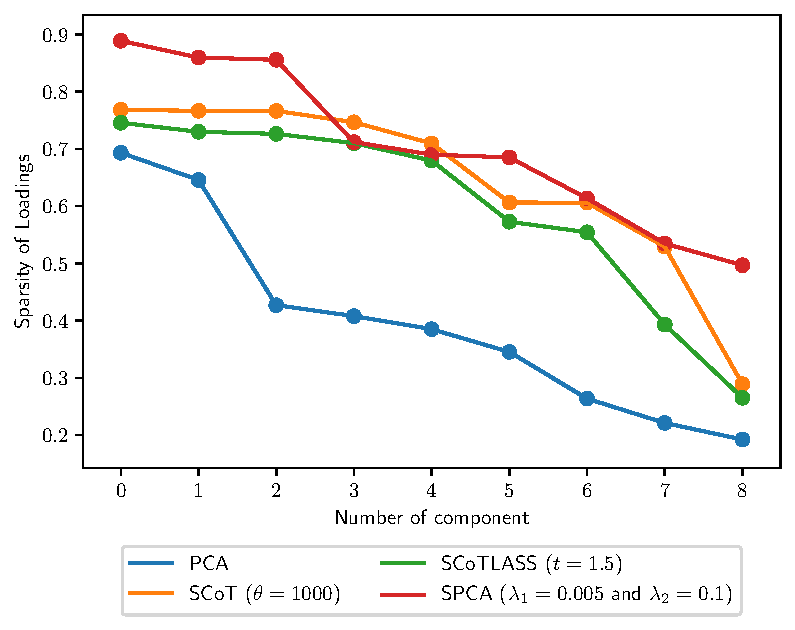
\includegraphics[scale = 0.5]{"../Figures/sparsityOfComponents.pdf"}
\end{figure}

\section*{Discussion}
We notice while PCA delivers us orthogonal principal components with optimal front-loaded explained variance, they are unintelligible. Over the years several sparse PCA algorithms have been introduced such as SCoT, SCoTLASS and SPCA. We find that all of them make a sparsity versus front-loaded variance trade-off. After comparing all models we conclude that SPCA comes out as the first his class with {\color{red} continue...}, but does not yield orthogonal components like the other options.\\

Since SPCA's components are correlated, an interesting future topic of research could be finding a way to transform these into orthogonal set of SPCA components. Moreover, while LARS and proximal gradient descent can be used to solve for a LASSO component, a lot of efficiency could be gained by a faster algorithm. As we tried working with a dataset of $>20k$ observations, we notice the many limitations these wide dataset enforce on PCA methods and their computability.
%Discussion: What did you find out? Do the results suggest any other interesting questions to explore?

% Pros of SCoT:
% - PCs are orthogonal
% - Computationally simpler than SCoTLASS
% Cons of SCoT:
% - difficult to tune 
%
% Pros of SCoTLASS:
% - PCs are orthogonal
% Cons of SCoTLASS:
% - Costly, requires random starts
% - difficult to tune
% - resulting PCs not as sparse as those resulting from other sparse PCA methods
% - selects at most n zero loadings (problematic when p >> n)
% Pros of SPCA:
%
% Cons of SPCA:
% - produces non orthogonal pcs

% Discussion points:
% - explore ways to create uncorrelated sparse PCAs
% - explore other optimization methods for SCoT and SCoTLASS that are more efficient
% - test methods with higher dimensional data sets

% References
\pagebreak
\bibliographystyle{apacite}
\bibliography{references}

% Appendix
\pagebreak
\appendix
\section*{Appendix}

\begin{algorithm}[H]
\SetAlgoLined
\KwResult{$V = [v_1,\ldots,v_k]$ where $\|v_j\|=1$}
$A_0 = Z$\;
\While{$\|A_{t+1} - A_{t}\|_F \ne 0$}{
    \For{$\beta_j$ in $B_{t+1}$}{
    $Y_j = X\alpha_j$\;
    $\beta_j = \arg\min_\beta \|Y_j - X\beta_j\|^2 + \lambda\|\beta\|^2 + \lambda_{1,j}\|\beta\|_1$\;
    }
    $X^TXB_{t+1}=UDV^T$\;
    $A_{t+1} = UV^T$\;
}
\For{$\alpha_j$ in $A$}{
$v_j = \alpha_j/\|\alpha_j\|$\;
}
\caption{General SPCA Algorithm}
\label{algo1:SPCA}
\end{algorithm}

\begin{table}[htpb!]
\caption{Variable descriptions}
\label{tab1:dta_vars}
\begin{center}
 \begin{tabular}{||c l||}
 \hline
Variable & Variable Description \\ [0.5ex] 
 \hline\hline
 $x_{1}$ & I0 - impedivity (ohm) at zero frequency \\ 
 \hline
 $x_{2}$ & 	PA500 - phase angle at 500 KHz \\
 \hline
 $x_{3}$ & HFS - high-frequency slope of phase angle \\
 \hline
 $x_{4}$ & DA - impedance distance between spectral ends \\
 \hline
 $x_{5}$ & AREA - area under spectrum \\
 \hline
 $x_{6}$ & 	A/DA - area normalized by DA \\
 \hline
 $x_{7}$ & MAX IP - maximum of the spectrum \\
 \hline
 $x_{8}$ & 	DR - distance between I0 and real part of the maximum frequency point \\
 \hline
 $x_{9}$ & P - length of the spectral curve \\ [1ex] 
 \hline
\end{tabular}
\end{center}
\end{table}

\begin{table}[htpb!]
    \centering
    \caption{SCoT Results for different parameters}
    \label{rstl:scot}
    \begin{tabular}{lrrrl}
\toprule
{} &  Explained Variance &  Concentration of EV &  Sparsity & Run time (sec) \\
\$\textbackslash lambda\$ &                     &                      &           &                \\
\midrule
10        &                 1.0 &             0.718422 &  0.280544 &             66 \\
100       &                 1.0 &             0.657778 &  0.292004 &             13 \\
500       &                 1.0 &             0.625546 &  0.410454 &              1 \\
1000      &                 1.0 &             0.335035 &  0.417198 &              1 \\
\bottomrule
\end{tabular}

\end{table}

\begin{table}[htpb!]
    \centering
    \caption{SCoTLASS Results for different parameters}
    \label{rstl:scotlass}
    \begin{tabular}{r|cccc}
\toprule
{} &  Concentration of EV &  Sparsity & Run Time (sec) \\
$t$ &                      &           &                \\
\midrule
1.0 &                 0.16 &      0.89 &              3 \\
1.2 &                 0.31 &      0.84 &             25 \\
1.5 &                 0.50 &      0.76 &             29 \\
1.6 &                 0.54 &      0.73 &             95 \\
2.0 &                 0.58 &      0.58 &             71 \\
\bottomrule
\end{tabular}

\end{table}

\begin{table}[htpb!]
    \centering
    \caption{SPCA Results for different parameters}
    \label{rstl:spca}
    \begin{tabular}{llrrrl}
\toprule
     &     &  Explained Variance &  Concentration of EV &  Sparsity & Run time (sec) \\
\$\textbackslash lambda\_1\$ & \$\textbackslash lambda\_2\$ &                     &                      &           &                \\
\midrule
1    & 0.1 &            0.777778 &             0.310112 &  0.589811 &             10 \\
10   & 0.1 &            0.777778 &             0.222222 &  0.666666 &              6 \\
100  & 0.1 &            0.679107 &             0.343493 &  0.631712 &              0 \\
1000 & 0.1 &            0.552005 &             0.620507 &  0.534239 &              0 \\
\bottomrule
\end{tabular}

\end{table}

\begin{figure}
\begin{subfigure}[htpb!]{0.49\textwidth}
    \centering
    \caption{Explained Variance for SCoT}
    \label{fig:EV_SCoT}
    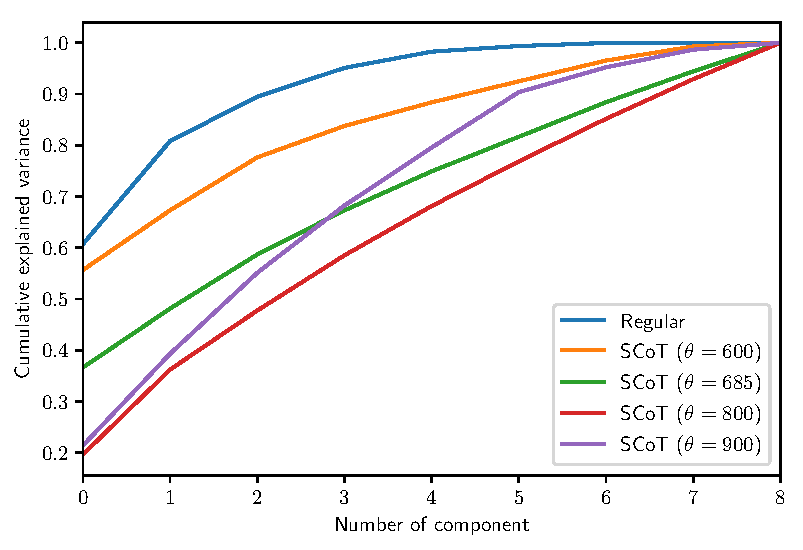
\includegraphics[scale = 0.5]{"../Figures/SCoT_comparison.pdf"}
\end{subfigure}
\begin{subfigure}[htpb!]{0.49\textwidth}
    \centering
    \caption{Explained Variance for SCoTLASS}
    \label{fig:EV_SCoTLASS}
    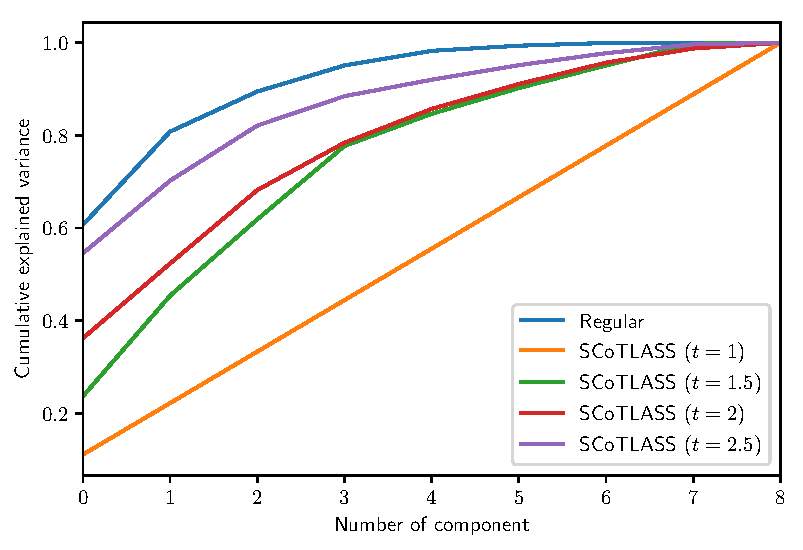
\includegraphics[scale = 0.5]{"../Figures/SCoTLASS_comparison.pdf"}
\end{subfigure}
\end{figure}



\end{document}